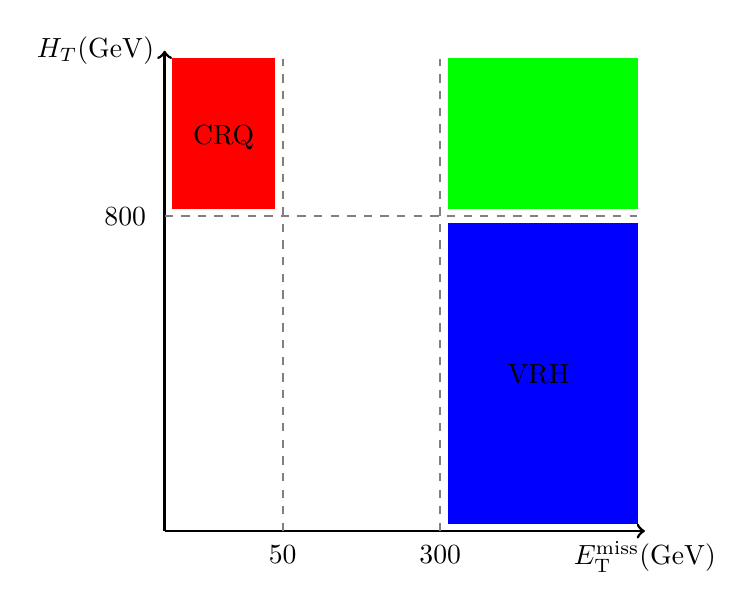
\begin{tikzpicture}[domain=0:4]

  \tikzstyle{region} = [fill]


  \draw[line width=1, ->] (0,0) -- (0,6.1) node[left] {$H_T (\mathrm{GeV})$};
  \draw[line width=1, ->] (0,0) -- (6.1,0) node[below] {$E_\mathrm{T}^\mathrm{miss} (\mathrm{GeV})$};

  %% \draw[gray, dashed, line width=0.8] (0, 2.5) -- (6, 2.5);
  \draw[gray, dashed, line width=0.8] (0, 4.0) -- (6, 4.0) node[black] at (-0.5,4.0) {800};
  \draw[gray, dashed, line width=0.8] (1.5, 0) -- (1.5, 6) node[black] at (1.5,-0.3) {50};
  \draw[gray, dashed, line width=0.8] (3.5, 0) -- (3.5, 6) node[black] at (3.5,-0.3) {300};

  \draw[green, region] (3.6,4.1) rectangle (6,6);
  \draw node at (4.75,5.0) {\large \SRH};

  \draw[red, region] (0.1,4.1) rectangle (1.4,6) ;
  \draw node at (0.75, 5) {CRQ};

  \draw[blue, region] (3.6,0.1) rectangle (6,3.9) ;
  \draw node at (4.75,2.) {VRH};

\end{tikzpicture}
